\documentclass[techrep,english]{ipsj} % techrep,

  \usepackage[nocompress]{cite}
  
  %\usepackage[dvips]{graphicx}
  \usepackage{latexsym}
  \usepackage{url}
  
  \usepackage{diagbox}
  
  \usepackage{tabu}
  \usepackage{footnote}
  \usepackage{tablefootnote}
  \usepackage{enumitem}
  \usepackage{times}
  \usepackage{float}
  \usepackage[binary-units=true,quotient-mode=fraction,table-auto-round]{siunitx}
  \sisetup{detect-all}
  \sisetup{range-phrase=--}
  \sisetup{range-units=single}
  \DeclareSIUnit\years{years}
  \usepackage{graphicx}
  \usepackage{subfigure}
  \usepackage{amsmath,amsfonts,amssymb}
  \usepackage{comment}
  \usepackage{multirow}
  \usepackage{bbding}
  \newcommand{\tabincell}[2]{\begin{tabular}{@{}#1@{}}#2\end{tabular}}
  \usepackage{times}
  \usepackage{soul}
  \usepackage{color}
  \usepackage{latexsym}
  \usepackage{booktabs,multirow,multicol}
  \usepackage{todonotes}
  \usepackage{multirow}
  \usepackage{comment}
  \usepackage{tabularx}
  \usepackage{url}
  
  \def\Underline{\setbox0\hbox\bgroup\let\\\endUnderline}
  \def\endUnderline{\vphantom{y}\egroup\smash{\underline{\box0}}\\}
  \def\|{\verb|}

\graphicspath{
    {resources/}
}


%\def\Underline{\setbox0\hbox\bgroup\let\\\endUnderline}
%\def\endUnderline{\vphantom{y}\egroup\smash{\underline{\box0}}\\}
%\def\|{\verb|}

\setcounter{volume}{26} % vol21=2013, 22=14, 23=15, 24=16, 25=17, 26=18
\setcounter{number}{1}
\setcounter{page}{1}

\usepackage[varg]{txfonts}%%!!
\makeatletter%
\input{ot1txtt.fd}
\makeatother%

\usepackage[hidelinks]{hyperref}
\usepackage[nameinlink,noabbrev,capitalise]{cleveref}

\begin{document}

\title{Accelerating Deep Neural Network Training on FPGAs Facilitating the Use of Variable Precision}

\affiliate{TiTech}{Tokyo Institute of Technology, 
Meguro, Tokyo 152--8550, Japan}
\affiliate{TUDelft}{Delft University of Technology, Mekelweg 2, 2628 CD Delft, Netherlands}

\author{Erwin de Haan}{TiTech,TUDelft}[e.r.dehaan@student.tudelft.nl]
\author{Artur Podobas}{TiTech}[podobas.a.aa@m.titech.ac.jp]
\author{Satoshi Matsuoka}{TiTech}[matsu@is.titech.ac.jp]

\begin{abstract}
The race for larger and deeper neural networks are leading researchers, vendors and practitioners to re-think architectural design decisions taken decades ago in hope to improve performance.
Among these decisions, reducing the numerical format is thought to be one of prime candidates to increasing performance.
Unfortunately, modern hardware has limited support for this, and the impact of modifying floating-point formats and its size remains shrouded in mystery.
To help investigate what the effects of varying the precision during deep-learning training are, first an architecture using reconfigurable hardware needs to be developed.
Through this work, we seek to accelerate arbitrary precision deep-learning training using Field-Programmable Gate-Arrays by leveraging Intel FPGA SDK for OpenCL.
Preliminary results show promise for implementations based on precisions or number formats that currently only have low performing implementations on conventional CPU and GPU hardware.
\end{abstract}

%\begin{keyword}
%Journal of Information Processing, \LaTeX, style files, ``Dos and
% Don'ts'' list
%\end{keyword}

\maketitle

\section{Introduction}
The present paper describes our efforts toward a customized and generalized framework for design-space exploration using alternative numerical floating-point formats through FPGAs.

The recent explosion in artificial intelligence – in particular that of deep neural networks based on backpropagation – has triggered a storm in the introduction and creation of specialized compute devices.
Commercial platforms such as Microsoft’s BrainWave~\cite{msbrainwave}, Google’s TPUs~\cite{googletpu}, and Fujitsu’s DLU~\cite{fujitsudlu} are all examples of specialized circuitry dedicated to low-power, high-performance Deep-Learning (DL) training and/or inference.
Meanwhile, existing general-purpose manufacturers are empowering their architecture with custom floating-point units that trade precision for performance, such as Intel’s Knights-Mill~\cite{knm} and NVIDIA’s Volta-100~\cite{volta100}.
It is clear that Artifical Intelligence and Deep-Learning will have a prioritized presence in modern architecture -- today and in the near future.

In the pursuit for faster and more energy efficient deep-learning architecture, there is a need to critically question the long-standing architectural design decision taken by computer architects decades ago.
One of the oldest design decision concerns the representation of real-valued numbers, otherwise known as the floating-point representation.
The IEEE-754 floating-point representation is one of the few relics still used unchanged in computing today.
Reducing the size of the floating-point representation can have dramatical (and positive) impacts on the performance: more compute per unit silicon, more compute per unit bandwidth, and lower power consumption.
Several alternatives to the IEEE-754 format are indeed emerging, such as Microsoft’s Deep-Learning format~\cite{msbrainwave}, Intel’s FlexPoint~\cite{intelflexpoint}, Google’s custom TPU format~\cite{tpuformat}, and Posits~\cite{posits}.

However, exploring the space around IEEE-754 floating-point representations and its alternatives pose a significant engineering problem: hardware and software infrastructure is to tightly coupled to the IEEE-754 standard that changing any part of it incurs a high engineering overhead.
One alternative is to simulate alternative floating-point representations in software, for example using soft-float or MPFR libraries~\cite{softfloat}, but the resulting performance is often several magnitudes lower than hardware implementations, limiting the size of the study conducted.
Furthermore, simulating alternative numerical formats in software are incapable of using any compiler optimizations, nor can they leverage the vector instruction often crucial to reach application performance in modern processors.
Porting the full software infrastructure stack is possible (and inevitable), but is a non-trivial effort that requires changes to the compiler, standard libraries and (possibly) the Application-Binary-Interface (e.g.\`calling convention).

A better way to explore floating-point representation is to leverage Field-Programmable Gate-Arrays (FPGAs).
An FPGA is a device consisting of several millions re-programmable look-up tables (LUTs) that together with programmable routers give a very malleable silicon substrate second only in performance to Application-Specific Integrate Circuits (ASICs).
Modern FPGAs can be clocked at several hundreds MHz, and contain enough compute to rival even Graphics-Processing Units (GPUs), making them ideal to study architectural design choices.
Furthermore, with the recent growth in popularity of High-Level Synthesis (HLS) tools, programming these devices can be as simple as writing C/C++ code, and delegate the software-to-hardware transformation effort to the compiler.

We contribute with the following:
\begin{itemize}
\item Proposed design for a generalized FPGA training architecture targeting variable numerical formats, and
\item Evaluation and analysis of core computation patterns, including FPGA resource utilization
\end{itemize}

The remainder of our paper is structure in the following way: \cref{sec:relwork} position our work against other, similar efforts.
\cref{sec:framework} gives a background to machine learning and FPGAs, and describes our proposed architecture.
\cref{sec:method} overviews our experimental methodology, and is followed by our preliminary results in \cref{sec:result}.
We conclude in \cref{sec:conclusion}.

\section{Related Work}\label{sec:relwork}
Field-Programmable Gate-Arrays (FPGAs) have extensively been used to probe and explore various architectural design decision, including those of deep-learning.
The large majority of existing work limit themselves to inference, primarily due to the simpler design layout (little intermediate data needs storing).
Levering FPGAs have allowed researchers to decrease the number of bits allocate to the numerical representation, going as far as inferring popular networks such as  AlexNET~\cite{krizhevsky2012imagenet} using as few as binary~\cite{shimoda2017all,umuroglu2017finn} (1-bit) weights.
Inferring networks that uses few bits to represents weights (called Quantized Neural Networks~\cite{courbariaux2016binarized}) requires subtle yet necessary changes to the training phase~\cite{binaryconnect,courbariaux2016binarized,zhou2016dorefa}.
Lately, modern deep-learning framework are having support for reduced precision training, some driven by leading FPGA vendors such as Xilinx~\cite{xilinxml}.
Dicecco et al.~\cite{dicecco2017fpga} are are working on a framework similar to ours – training neural networks using FPGAs while modifying the numerical format.
Their work primary focus on the IEEE-754 format and convolution layers where-as we aspire to include alternative format such as posits~\cite{posits}.
Using posits in deep-learning was intended the focus of Langroudi et al.~\cite{langroudi2018deep}’s work; however, they only compared the performance against fixed-point and only \textit{stored} the weights as posit (the computation was still done using IEEE-754).

FPGAs are not unique to vary the numerical precision of deep neural networks, and several ASICs have been produced for quantized neural networks.
Most of these focus only on inference (for embedded deployment)  for low-power embedded domains; these include YodaNN~\cite{yodann}, BinaryEYE~\cite{binaryeye} and ChipMunk~\cite{chipmunk}; these ASICs were shown to consume up-to two magnitudes low power compared to similar FPGA solutions.

Commercially most vendors do support some form of reduced precision mode.
Intel’s Knight’s Milll~\cite{knm} architecture replaces one of the AVX-512 vector units of Knight’s Landing with a Vector Neural Network Instruction (VNNI) unit, capable of performing dot-products in a mixed IEEE-754 16-bit and 32-bit mode.
A similar process (reduced precision multiplication, full precision accumulation) is also applied in NVIDIA’s Volta-100 line GPUs.
These mixed-precision units drastically improve the Artificial-Intelligence compute capabilities (AI-FLOPs) of modern systems, trading silicon resource for increased compute with arguable small impact on training performance.
Vendors also embrace drastically different formats, notably in Intel’s NERVANA~\cite{nervana} (likely where FlexPoint~\cite{intelflexpoint} is used) and Google’s TPU~\cite{tpuformat} (which have more bits in the exponent compared to the mantissa).


\section{A FPGA-based CNN Framework}\label{sec:framework}
\subsection{Field-Programmable Gate-Arrays}
%Small intro to FPGAs.
FPGAs can be used for a great variety of things, from accelerating computational algorithms to implementating a hardware design before taping out full chip.
They are devices that can represent reconfigurable hardware.

The fabric they are made up of consists of vast arrays of switches and other routing hardware to connect all the functional elements, like multipliers, block RAM and look up tables, in any way possible.
This makes them very suitable for the research described in this paper.
It gives total freedom to design a hardware implementation to explore algorithms in a hardware setting.

\subsection{Neural Networks}
Intro to neural networks.
%TODO

\subsection{FPGA NN Framework}
A small framework was built, consisting of multiple kernels.
One simple forward propagation kernel with optional Relu activation function integrated and a forward softmax kernel.
\subsubsection{Design overview}
\Cref{fig:block-diagram} shows a overview of the system.
The backwards kernels are a work in progress, so for now we use an external training script.
The host code, written in python, does a kernel call for every layer.

\begin{figure*}[ht]
  \centering
  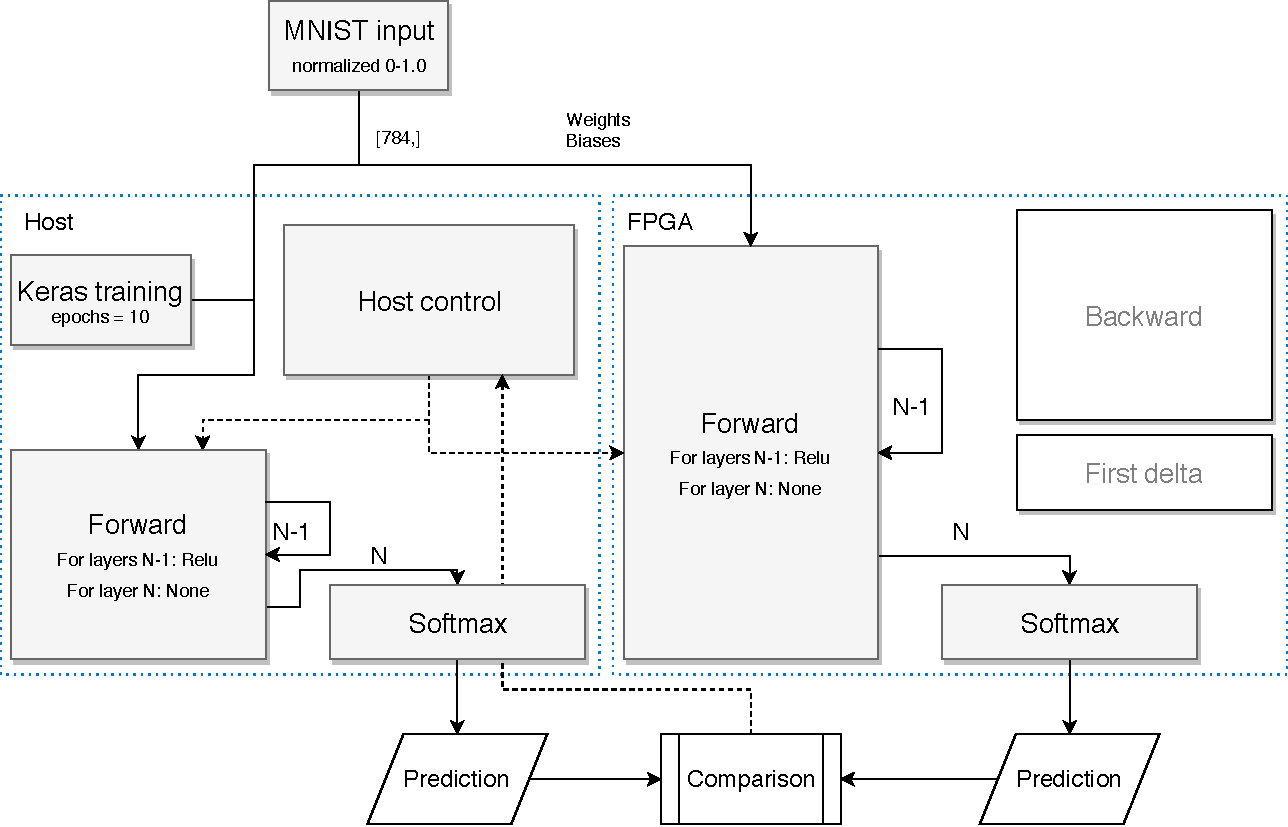
\includegraphics[width=\linewidth]{block-diagram.pdf}
  \caption{Block diagram of implementation}\label{fig:block-diagram}
\end{figure*}

\subsubsection{Design details}
All weight matrices are transposed in memory.
The main inference is done using an blocking implementation of the matrix multiplication.
So a block is fetched from the activations and the wieghts and place in the block RAM on the FPGA.
The block RAM is much faster then the global memory.
This speeds up through put by a large margin.
Block RAM is equivalent to the shared or local memory of contemporary GPUs.

\subsubsection{Design decisions}
Decisions taken while designing.
The *why* we did as we did.

\section{Methodology}\label{sec:method}
\subsection{Experimental Platform}
The software versions and hardware configuration are shown in respectively \cref{tab:software-versions} and \cref{tab:test-hardware}.
All kernels were compiled with \texttt{-O3 -fp-relaxed}.
\texttt{-fp-relaxed} gives the compiler some more freedom with the order of operations, this gives about a \SIrange{10}{15}{\percent} performance benefit without changing the numerical output.
\begin{table}[h]
  \centering
  \caption{Used software versions}\label{tab:software-versions}
  \begin{tabular}{ll}
    \toprule
    \textbf{Software} & \textbf{Version} \\
    \midrule
    Python & v3.6.3 \\
    Keras & v2.2.0 \\
    TensorFlow & v1.8.0 \\
    Intel Quartus & v17.1.0 \\
    \bottomrule
  \end{tabular}
\end{table}
\begin{table}[h]
  \centering
  \caption{Test hardware}\label{tab:test-hardware}
  \begin{tabular}{ll}
    \toprule
    \textbf{Hardware} & \textbf{Configuration} \\
    \midrule
    Intel i7-3930K & \SI{3.20}{\giga\hertz} \\
    Host RAM & DDR3-\SI{1333}{\mega\hertz} Dual Channel \\
    Arria 10 (x1) & Nallatech 510T \\
    \bottomrule
  \end{tabular}
\end{table}

\subsection{Network Tested + Data-set}
The used example network is a simple multilayer perceptron.
The main dataset used was MNIST with a layer depth of 1 and a first layer output size of 128.
So in total a two layer network.
The data set was trained using the first \num{50000} images from the MNIST dataset.
The last \num{10000} images are used as the test data set.
Training was done using a batch size of 128.
The CPU code was implemented using the NumPy array.dot function.

\section{Results}\label{sec:result}
The host (numpy based) code benchmarked at \num{41} GFLOPS for simple inference.
Our first naive implementation clocked about \num{2.5} GFLOPS for this problem size.
The results for the different final FPGA kernels are shown in \cref{tab:kernel-performance}.

\begin{table}[h]
  \centering
  \caption{FPGA Kernel performance}\label{tab:kernel-performance}
  \begin{tabular}{ll}
    \toprule
    \textbf{Block size} & \textbf{GFLOPS}  \\
    \midrule
    128x128 & \num{0}  \\
    100x100 & \num{0} \\
    84x84 & \num{0}  \\
    64x64 & \num{14.3}  \\
    32x32 & \num{0}  \\
    16x16 & \num{4.1}  \\
    \bottomrule
  \end{tabular}
\end{table}


\subsection{FPGA Resource Utilization}
The kernel resource utilization is shown in \cref{tab:fpga-util}.

\begin{table}[h]
  \centering
  \caption{FPGA Hardware utilisation for different blocksizes}\label{tab:fpga-util}
  \begin{tabular}{lllll}
    \toprule
    \textbf{Block size} & \textbf{Logic} & \textbf{DSPs} & \textbf{RAMs} & \textbf{Fmax} \\
    \midrule
    128x128 & \SI{0}{\percent} & \SI{0}{\percent} & \SI{0}{\percent} & \SI{0}{\mega\hertz}  \\
    100x100 & \SI{0}{\percent} & \SI{0}{\percent} & \SI{0}{\percent} & \SI{0}{\mega\hertz}  \\
    84x84 & \SI{0}{\percent} & \SI{0}{\percent} & \SI{0}{\percent} & \SI{0}{\mega\hertz}  \\
    64x64 & \SI{33}{\percent} & \SI{10}{\percent} & \SI{68}{\percent} & \SI{172.8}{\mega\hertz}  \\
    32x32 & \SI{0}{\percent} & \SI{0}{\percent} & \SI{0}{\percent} & \SI{0}{\mega\hertz}  \\
    16x16 & \SI{17}{\percent} & \SI{3}{\percent} & \SI{30}{\percent} & \SI{209.16}{\mega\hertz}  \\
    \bottomrule
  \end{tabular}
\end{table}

\subsection{Training Performance}
The accuracy after training on the CPU using Keras is \SI{97.9}{\percent}.
The FPGA gets slightly different floaing point results due to rounding differences but is matches the accuracy.

\section{Conclusion}\label{sec:conclusion}


\begin{thebibliography}{99}

\bibitem{msbrainwave}
  Chung, Eric and Fowers, Jeremy and Ovtcharov, Kalin and Papamichael, Michael and Caulfield, Adrian and Massengill, Todd and Liu, Ming and Lo, Daniel and Alkalay, Shlomi and Haselman, Michael and others:
  Serving DNNs in Real Time at Datacenter Scale with Project Brainwave:
  {\it IEEE Micro},
  vol.
38, number.
2, pp 8--20, 2018

\bibitem{googletpu}
  Google Blog (online):
  Google Supercharges Machine Learning Tasks with TPU Custom Chip,
  {\it https://cloudplatform.googleblog.com/2016/05/Google-supercharges-machine-learning-tasks-with-custom-chip.html}
  Accessed: 2018-06-25

\bibitem{fujitsudlu}
  Fujitsu:
  Post-K Development and Introducing DLU - Fujitsu,
  {\it http://www.fujitsu.com/global/Images/post-k-development-and-introducing-dlu.pdf},
  2016

\bibitem{knm}
  Bradford, Dennis and Chinthamani, Sundarama and Corbral, Jesus and Hassan, Adhiraj and Janik, Ken:
  Knights Mill: Intel Xeon Phi Processor for Machine Learning,
  {\it Hot Chips 2017},
  2017
  
\bibitem{volta100}
  NVIDIA:
  Artificial Intelligence Architecture,
  {\it https://www.nvidia.com/en-us/data-center/volta-gpu-architecture/},
  Accessed: 2018-06-25

\bibitem{intelflexpoint}
  Koster, Urs and Webb, Tristan and Wang, Xin and Nassar, Marcel and Bansal, Arjun K and Constable, William and Elibol, Oguz and Gray, Scott and Hall, Stewart and Hornof, Luke and others:
  FlexPoint: An Adaptive Numerical Format for Efficient Training of Deep Neural Networks,
  {\it Advances in Neural Information Processing Systems},
  pp 1742--1752, 2017

\bibitem{tpuformat}
  The Next Platform:
  Tearing Apart Google’s TPU 3.0 AI CoProcessor,
  {\it https://www.nextplatform.com/2018/05/10/tearing-apart-googles-tpu-3-0-ai-coprocessor},
  Accessed: 2018-06-25
    
\bibitem{posits}
  Gustafson, John L and Yonemoto, Isaac T:
  Beating Floating Point at its Own Game: Posit Arithmetic,
  {\it Supercomputing Frontiers and Innovations},
  vol.
4, num.
2, pp 71--86, 2017

\bibitem{softfloat}
  Fousse, Laurent and Hanrot, Guillaume and Lef{\`e}vre, Vincent and P{\'e}lissier, Patrick and Zimmermann, Paul:
  MPFR: A Multiple-Precision Binary Floating-Point Library with Correct Rounding,
  {\it ACM Transactions on Mathematical Software (TOMS)},
  vol.
32, num.
2, pp.
13, 2007


\bibitem{langroudi2018deep}
  Langroudi, Seyed HF and Pandit, Tej and Kudithipudi, Dhireesha:
  Deep Learning Inference on Embedded Devices: Fixed-Point vs Posit,
  {\it arXiv preprint arXiv:1805.08624},
  2018

\bibitem{nervana}
  Intel:
  Intel Nervana Neural Network Processor,
  {\it https://ai.intel.com/intel-nervana-neural-network-processor/},
  Access: 2018-06

\bibitem{xilinxml}
  Xilinx:
  Xilinx ML Suite,
  {\it https://www.xilinx.com/applications/megatrends/machine-learning.html},
  Accessed: 2018-16

\bibitem{krizhevsky2012imagenet}
  Krizhevsky, Alex and Sutskever, Ilya and Hinton, Geoffrey E:
  Imagenet classification with deep convolutional neural networks,
  {\it Advances in neural information processing systems},
  pp 1097–1105, 2012

\bibitem{binaryconnect}
  Courbariaux, Matthieu and Bengio, Yoshua and David, Jean-Pierr:
  Binaryconnect: Training deep neural networks with binary weights during propagations,
  {\it Advances in neural information processing systems},
  pp 3123–3131, 2015

\bibitem{zhou2016dorefa}
  Zhou, Shuchang and Wu, Yuxin and Ni, Zekun and Zhou, Xinyu and Wen, He and Zou, Yuheng:
  DoReFa-Net: Training low bitwidth convolutional neural networks with low bitwidth gradients
  {\it  arXiv preprint arXiv:1606.06160},
  2016

\bibitem{yodann}
  Andri, Renzo and Cavigelli, Lukas and Rossi, Davide and Benini, Luca:
  YodaNN: An Architecture for Ultralow Power Binary-Weight CNN Acceleration
  {\it IEEE Transactions on Computer-Aided Design of Integrated Circuits and Systems},
  vol.
37, num.
1, pp 48–60, 2018

\bibitem{binaryeye}
  Moons, Bert and Bankman, Daniel and Yang, Lita and Murmann, Boris and Verhelst, Marian:
  BinarEye: An always-on energy-accuracy-scalable binary CNN processor with all memory on chip in 28nm CMOS,
  {\it Custom Integrated Circuits Conference (CICC), 2018 IEEE},
  pp 1–4, 2018


\bibitem{chipmunk}
  Conti, Francesco and Cavigelli, Lukas and Paulin, Gianna and Susmelj, Igor and Benini, Luca:
  Chipmunk: A systolically scalable 0.9 mm 2, 3.08 Gop/s/mW@ 1.2 mW accelerator for near-sensor recurrent neural network inference,
  {\it Custom Integrated Circuits Conference (CICC), 2018 IEEE},
  pp 1–4, 2018

\bibitem{dicecco2017fpga}
  DiCecco, Roberto and Sun, Lin and Chow, Paul:
  FPGA-based training of convolutional neural networks with a reduced precision floating-point library,
  {\it  Field Programmable Technology (ICFPT), 2017 International Conference on},
  pp 239–242, 2016

\bibitem{shimoda2017all}
  Shimoda, Masayuki and Sato, Shimpei and Nakahara, Hiroki:
  All binarized convolutional neural network and its implementation on an FPGA,
  {\it  Field Programmable Technology (ICFPT), 2017 International Conference on},
  pp 291–294, 2017

\bibitem{umuroglu2017finn}
  Umuroglu, Yaman and Fraser, Nicholas J and Gambardella, Giulio and Blott, Michaela and Leong, Philip and Jahre, Magnus and Vissers, Kees:
  Finn: A framework for fast, scalable binarized neural network inference,
  {\it  Proceedings of the 2017 ACM/SIGDA International Symposium on Field-Programmable Gate Arrays},
  pp 65–74, 2017


\bibitem{courbariaux2016binarized}
  Courbariaux, Matthieu and Hubara, Itay and Soudry, Daniel and El-Yaniv, Ran and Bengio, Yoshua:
  Binarized neural networks: Training deep neural networks with weights and activations constrained to+ 1 or-1,
  {\it arXiv preprint arXiv:1602.02830},
  2016
  
\end{thebibliography}  

\end{document}
